\newpage
\subsection{Emotion Mapping to A-V Plan}\label{sec:emotion-mapping}

After collecting the emotional data, we need to represent these emotions in the arousal-valence (A-V) space. To do this, we convert the categorical emotion labels (like happy, sad, angry) into numerical coordinates on the A-V plane.

Arousal and valence are two important dimensions in emotion research. Valence shows how pleasant or unpleasant a feeling is, while arousal shows how calm or excited the feeling is. The \textbf{Circumplex Model of Affect}, proposed by \cite{russell1980circumplex}, is widely used to represent this concept. It places emotions in a circular 2D space, where each emotion is mapped according to its valence and arousal values. For example, happiness is usually high in both valence and arousal, while sadness is low in both.

However, the original model does not give exact numbers for each emotion. So, for this research, we use the numerical coordinates for emotions proposed by \cite{paltoglou2012seeing}. Their work gives us empirically validated A-V values for a set of common emotions. These values are especially suitable for computational models and were derived from large-scale emotion analysis in text data, which makes them practical and tested.

We selected these values for a few key reasons:

\begin{itemize}
    \item \textbf{Empirical Validation:} The values are based on real data and experiments, not just theory.
    \item \textbf{Computational Use:} The values are already tested in affective computing systems.
    \item \textbf{Standardization:} Using known values makes our system easier to compare with other studies.
    \item \textbf{Dimensional Mapping:} They fit well with our aim to measure emotions on a scale, not just labels.
\end{itemize}


Figure~\ref{fig:circumplex_model} shows the general circular A-V model proposed by Russell, and Figure~\ref{fig:emotion_coordinates} presents the exact coordinates used in this study, based on the work of Paltoglou and Thelwall.


\begin{figure}[H]
    \centering
    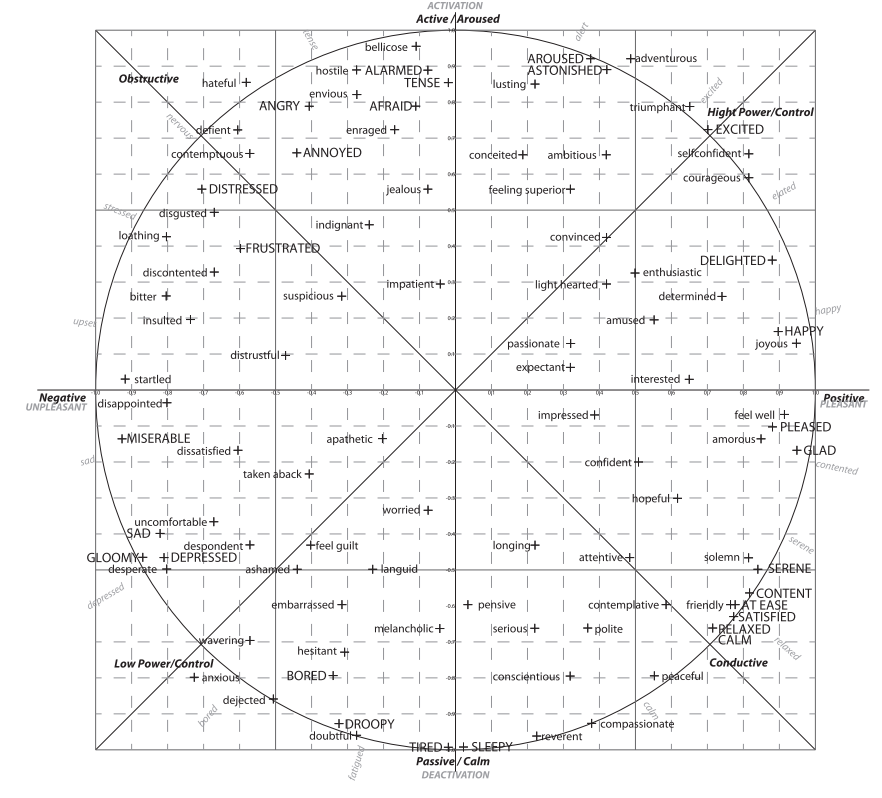
\includegraphics[width=0.6\textwidth]{img/chapter_03/circumplex_model.png}
    \caption{Circumplex Model of Affect \cite{russell1980circumplex}. This circular model shows how emotions are distributed in a two-dimensional space using arousal and valence.}
    \label{fig:circumplex_model}
\end{figure}

\begin{figure}[H]
    \centering
    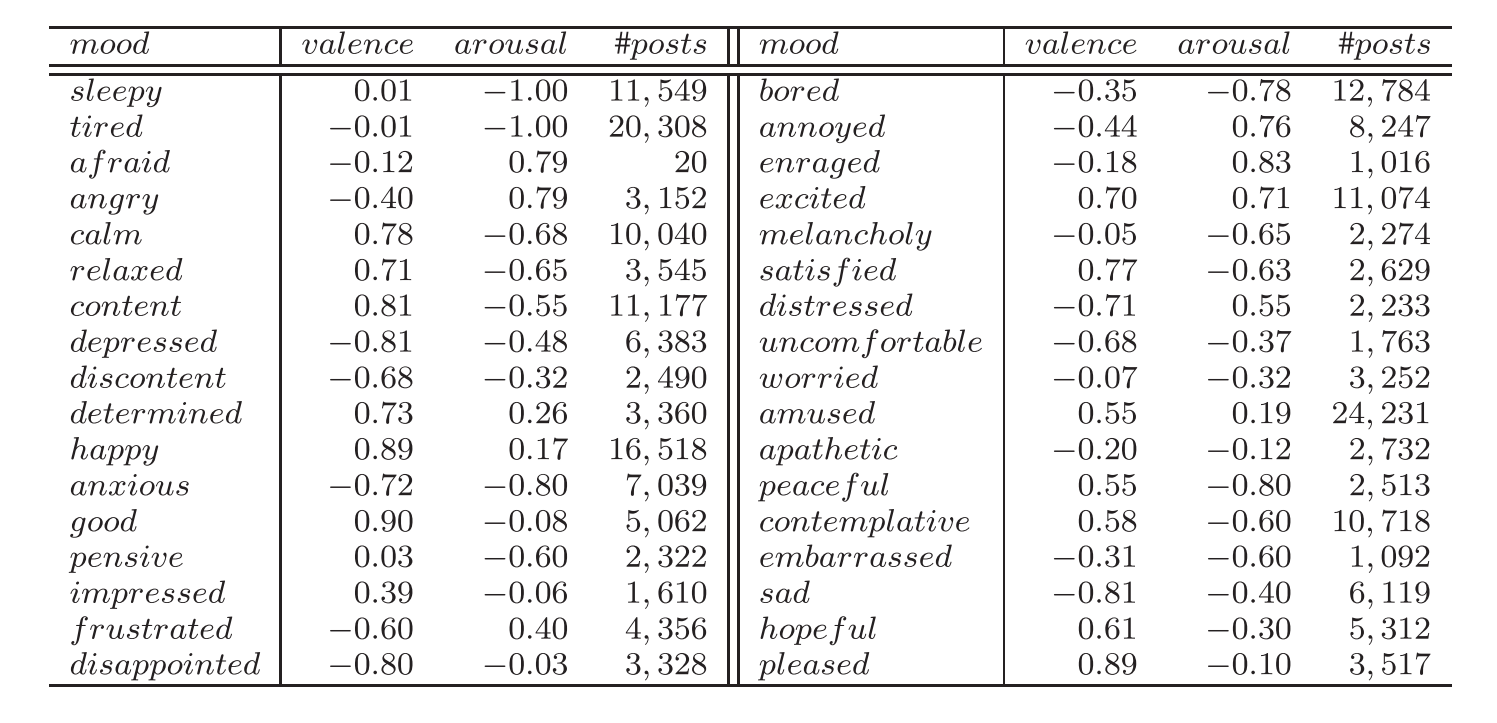
\includegraphics[width=0.8\textwidth]{img/chapter_03/emotion_coordinates_table.png}
    \caption{Emotion coordinates adapted from \cite{paltoglou2012seeing}. These values are used in this study to map categorical emotions to A-V values.}
    \label{fig:emotion_coordinates}
\end{figure}


\begin{itemize}
    \item \textbf{Happy}: Valence = 0.89, Arousal = 0.17
    \item \textbf{Angry}: Valence = -0.40, Arousal = 0.79
    \item \textbf{Sad}: Valence = -0.81, Arousal = -0.40
    \item \textbf{Boredom}: Valence = -0.35, Arousal = -0.78
    \item \textbf{Calm}: Valence = 0.78, Arousal = -0.68
\end{itemize}

To show different emotional intensities, we applied a \textbf{linear scaling method}. Here, each emotion starts at the neutral point $(0,0)$, and intensity levels from 1 to 10 move the emotion point closer to its full coordinate. This follows the idea that emotional intensity changes smoothly in a straight line from neutral to peak intensity, which is also supported in literature \cite{posner2005circumplex}.

To calculate the valence and arousal coordinates at any intensity level \( i \), where \( i \in \{1, 2, ..., 10\} \), the following formula is used:

\begin{equation}
\text{Valence}_{i} = \frac{\text{Valence}_{\text{max}} \times i}{10}, \quad
\text{Arousal}_{i} = \frac{\text{Arousal}_{\text{max}} \times i}{10}
\end{equation}

Where:

\begin{itemize}
    \item \( \text{Valence}_{\text{max}} \) is the valence value at maximum intensity (level 10)
    \item \( \text{Arousal}_{\text{max}} \) is the arousal value at maximum intensity (level 10)
    \item \( i \) is the current intensity level
\end{itemize}

This formula creates a straight path from the neutral point \((0,0)\) to the maximum intensity point for each emotion. For example:

\begin{itemize}
    \item At intensity level 1, the coordinates are 10\% of the maximum
    \item At level 5, they are 50\%
    \item At level 10, the full intensity is reached
\end{itemize}


Table~\ref{tab:emotion_coordinates} presents the standardized valence and arousal coordinates for five testing emotions across different intensity levels scale from 1 to 10. 

\begin{table}[H]
    \centering
    \caption{Emotion Intensity Coordinates Based on Paltoglou \& Thelwall (2012)}
    \begin{tabular}{p{0.8cm}|cc|cc|cc|cc|cc}
    
    \textbf{Int.} & \multicolumn{2}{c|}{\textbf{Happy}} & \multicolumn{2}{c|}{\textbf{Angry}} & \multicolumn{2}{c|}{\textbf{Sad}} & \multicolumn{2}{c|}{\textbf{Boredom}} & \multicolumn{2}{c}{\textbf{Calm}} \\
    
    & Val & Aro & Val & Aro & Val & Aro & Val & Aro & Val & Aro \\
    \hline
    1 & 0.089 & 0.017 & -0.040 & 0.079 & -0.081 & -0.040 & -0.035 & -0.078 & 0.078 & -0.068 \\
    2 & 0.178 & 0.034 & -0.080 & 0.158 & -0.162 & -0.080 & -0.070 & -0.156 & 0.156 & -0.136 \\
    3 & 0.267 & 0.051 & -0.120 & 0.237 & -0.243 & -0.120 & -0.105 & -0.234 & 0.234 & -0.204 \\
    4 & 0.356 & 0.068 & -0.160 & 0.316 & -0.324 & -0.160 & -0.140 & -0.312 & 0.312 & -0.272 \\
    5 & 0.445 & 0.085 & -0.200 & 0.395 & -0.405 & -0.200 & -0.175 & -0.390 & 0.390 & -0.340 \\
    6 & 0.534 & 0.102 & -0.240 & 0.474 & -0.486 & -0.240 & -0.210 & -0.468 & 0.468 & -0.408 \\
    7 & 0.623 & 0.119 & -0.280 & 0.553 & -0.567 & -0.280 & -0.245 & -0.546 & 0.546 & -0.476 \\
    8 & 0.712 & 0.136 & -0.320 & 0.632 & -0.648 & -0.320 & -0.280 & -0.624 & 0.624 & -0.544 \\
    9 & 0.801 & 0.153 & -0.360 & 0.711 & -0.729 & -0.360 & -0.315 & -0.702 & 0.702 & -0.612 \\
    10 & 0.890 & 0.170 & -0.400 & 0.790 & -0.810 & -0.400 & -0.350 & -0.780 & 0.780 & -0.680 \\
    
    \end{tabular}
    \label{tab:emotion_coordinates}
\end{table}